% VUT FIT
% IUS 2016/2017
% Projekt - Model informacniho systemu
% Soubor: model_informacniho_systemu.tex
% Autor: Vladimir Dusek, xdusek27 (1BIT)
% Datum: 27. 11. 2016

\documentclass[12pt,a4paper,oneside]{article}
\usepackage[utf8]{inputenc}
\usepackage[czech]{babel}
\usepackage[T1]{fontenc}
\usepackage{a4wide}
\usepackage{amsmath,amsfonts,amssymb}
\usepackage{graphicx}
\usepackage{pdfpages}

\begin{document}

%%%%%%%%%%%%%%%%%%%%%%%%%%%%%%%%%%%%%%%%%%%%%%%%%%%%%%%%%%%%%%%%%%%%%%%%%%%%%%%%%%%%%%%%%%%%%%%%%%%%%%%%

\begin{center}
\begin{LARGE}

\textsc{Vysoké učení technické v Brně}

\medskip
Fakulta informačních technologií 

\vspace{3cm} 
\textsc{Úvod do softwarového inženýrství}

\medskip
2016/2017

\vspace{3cm}
Projekt - Model informačního systému

\medskip
\textbf{Zadání č. 36 - Lístky na vlak}

\end{LARGE}
\end{center}

\begin{large}
\vfill 
Vladimír Dušek (xdusek27)
\hfill Brno, 25. listopadu 2016
\end{large}

\clearpage

%%%%%%%%%%%%%%%%%%%%%%%%%%%%%%%%%%%%%%%%%%%%%%%%%%%%%%%%%%%%%%%%%%%%%%%%%%%%%%%%%%%%%%%%%%%%%%%%%%%%%%%%

\begin{LARGE}
\begin{center}
\textbf{Zadání}
\end{center}
\end{LARGE}

\bigskip
\noindent
Navrhněte fragment informačního systému pro prodej lístků na vlakové spoje. Systém bude umět odpovědět na dotazy typu jakou trasou zvolený spoj jede, jaké jsou vzdálenosti (časové) mezi zastávkami, jaký typ vlaku jede, průměrné zpoždění vlaku, apod. Doba přepravy mezi dvěma zastávkami může být různá v závislosti na typu vlaku. Uvažujte více společností provozujících vlakové spoje. Různé vlaky nabízí různé služby (jídelní vůz, spací vůz, přeprava kol, apod.), za jejich využití se platí pevně daný příplatek. Dostupnost služby či velikost příplatku se liší v závislosti na vlaku. Na základě uložených dat by si měl uživatel být schopen vyhledat spoj mezi dvěma zastávkami, zjistit dostupné služby a zjistit výslednou cenu přepravy. Uživatel si může přes internet koupit (a zrušit již zakoupenou) jízdenku a procházet historii svých jízdenek.

\clearpage

%%%%%%%%%%%%%%%%%%%%%%%%%%%%%%%%%%%%%%%%%%%%%%%%%%%%%%%%%%%%%%%%%%%%%%%%%%%%%%%%%%%%%%%%%%%%%%%%%%%%%%%%%%

\begin{LARGE}
\begin{center}
\textbf{Use case diagram}
\end{center}
\end{LARGE}

\bigskip \bigskip \bigskip
\begin{figure}[htb]
	\centering
	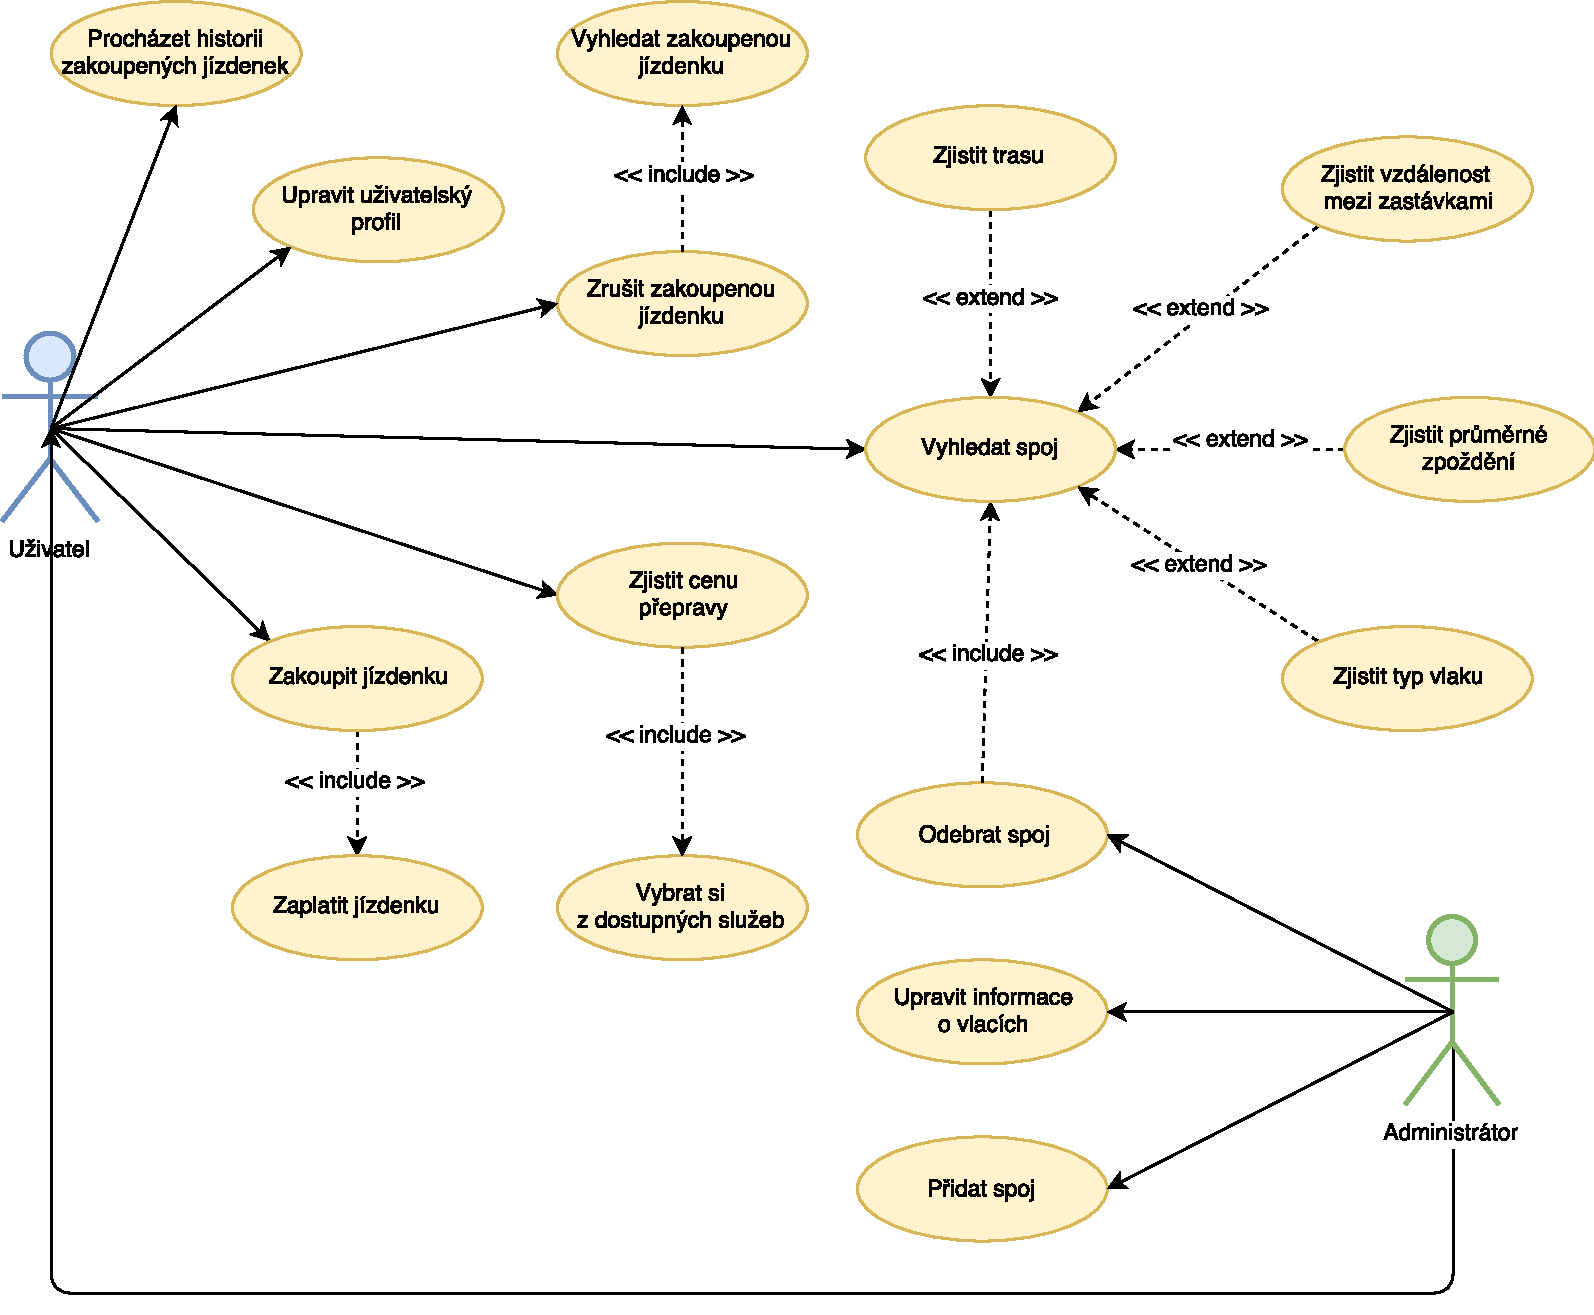
\includegraphics[width=0.8\hsize]{use_case.pdf}
\end{figure}

\clearpage

%%%%%%%%%%%%%%%%%%%%%%%%%%%%%%%%%%%%%%%%%%%%%%%%%%%%%%%%%%%%%%%%%%%%%%%%%%%%%%%%%%%%%%%%%%%%%%%%%%%%%%%%%%

\begin{LARGE}
\begin{center}
\textbf{Entity-relationship diagram}
\end{center}
\end{LARGE}

\bigskip \bigskip \bigskip
\begin{figure}[htb]
	\centering
	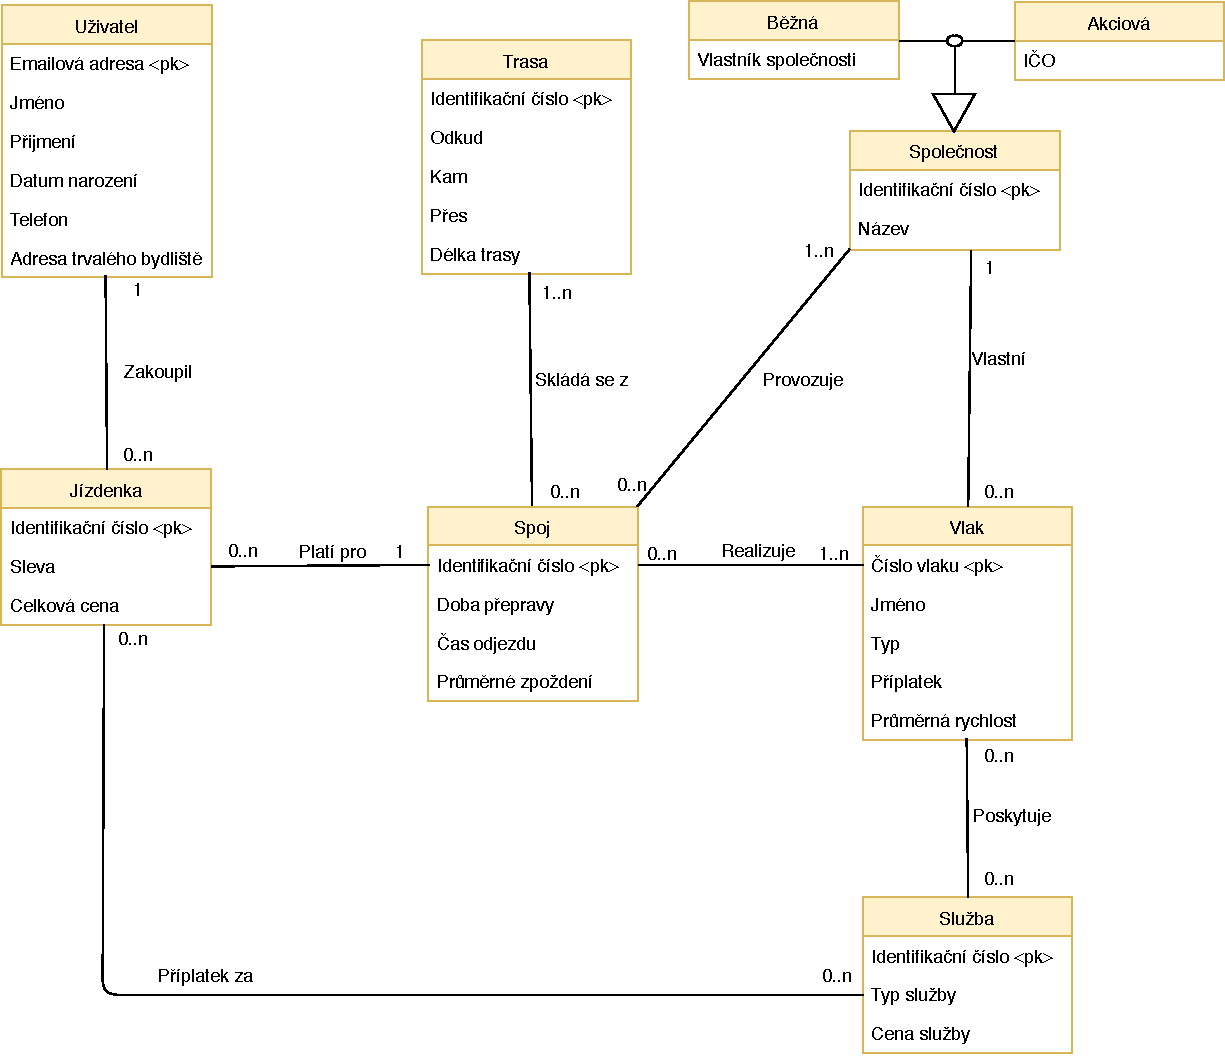
\includegraphics[width=0.8\hsize]{erd.pdf}
\end{figure}

\clearpage

\end{document}
